\section{Derivada de la función logística}

Para poder calcular el gradiente, primero debemos ver la derivada de la función logística. Recordemos en la siguiente figura 
como se ve la función logística.

\begin{figure}[h]
 \centering
 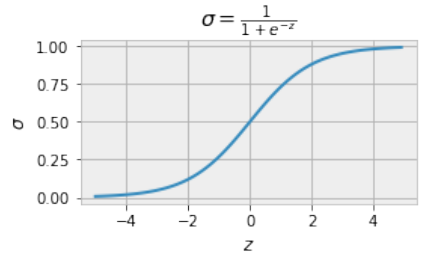
\includegraphics[scale=0.5]{../Figuras/devLog1.png}
 \caption{Gráfica función logistica.}
 \label{fig:graficaLog1}
\end{figure}
\begin{figure}[h]
    \centering
    \subfloat[Función logistica.]{
            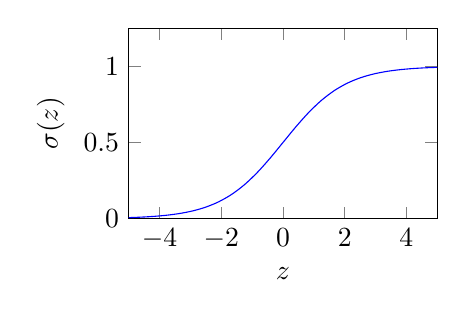
\begin{tikzpicture}
            \begin{axis}[width=5.5cm,height=4cm,ylabel=$\sigma(z)$,xlabel=$z$,ymin=0,ymax=1.25,xmin=-5,xmax=5]
                \addplot[blue,smooth] {1/(1+exp(-x))};
                %\addlegendentry{$y = \dfrac{1}{1+e^{-x}}$}
            \end{axis}
        \end{tikzpicture}
    }
        \caption[Funciones de activación]{}
        \label{fig:sigmoid-tanh}
\end{figure}


La función logistica estandar centrada en el origen como en la figura \ref{fig:graficaLog1} se escribe de la siguiente forma:
\begin{equation}
 \sigma(z) = \dfrac{1}{1+e^{-(z)}}
\end{equation}

Los siguientes calculos son realizados para un solo perceptrón, en concreto uno de salida, donde este está recibiendo los datos de salida de neuronas en la capa oculta, así el factor $z$ que está recibiendo la función, es la combinación lineal de los valores de entrada multiplicados por los pesos asignados para esté perceptrón y sumados todos. Entonces $z = X\Theta = [X_0\theta_0 +X_1\theta_1+...+X_n\theta_n]$. Así nuestra función queda de la siguiente forma:

\begin{equation}
  \sigma_{\Theta}(X) = \dfrac{1}{1+e^{-X\Theta}}
\end{equation}

Entonces vamos a calcular la derivada de esta función con respecto a cualquiera de estos parámetros $i$ de $z$.
Por la regla de la cadena comenzamos calculando la derivada queda de la siguiete forma:

\begin{equation}
 \dfrac{\partial\sigma}{\partial\theta_{i}}= -\dfrac{1}{(1-e^{-X\Theta})^2}e^{-x\Theta}(-x_{i})
\end{equation}

Reescribiendo la misma derivada con un poco de algebra nos queda de la siguiete forma:
\begin{equation}
 \dfrac{\partial\sigma}{\partial\theta_{i}}= \dfrac{1}{1+e^{-X\Theta}}  \dfrac{e^{-x\Theta}}{1+e^{x\Theta}} x_{i}
\end{equation}

Con la reescritura anterior nos damos cuenta que tenemos la función sigma en uno de los productos así que procedemos a sustituirlo y a sumar y restar unos unos. Así obteniendo lo siguiente:
\begin{equation}
 \dfrac{\partial\sigma}{\partial\theta_{i}}= \sigma_{\Theta}(X)\dfrac{e^{-x\Theta}-1+1}{1+e^{x\Theta}} x_{i}
\end{equation}

Vamos a separar a conveniencia los terminos de la siguiente forma:
\begin{equation}
 \dfrac{\partial\sigma}{\partial\theta_{i}}= \sigma_{\Theta}(X)
 \left( \dfrac{1+e^{-x\Theta}}{1+e^{-x\Theta}}-\dfrac{1}{1+e^{-x\Theta}}\right)x_{i}
\end{equation}

Así sustituyendo con la función sigmoide y llevando a uno, llegamos a lo siguiente:
\begin{equation}
 \dfrac{\partial\sigma}{\partial\theta_{i}}= \sigma_{\Theta}(X)
 (1- \sigma_{\Theta}(X))x_{i}
\end{equation}

Entonces lo que tenemos es una propiedad bastante interesante de la función logística. Se está calculando la derivada de sigma con respecto al exponente osea que sería:
Entonces lo que vemos es que la derivada de la sigmoide es la sigmoide por uno menos la sigmoide:

\begin{equation}
 \dfrac{\partial\sigma}{\partial\theta_{z}}= \sigma(1- \sigma)
\end{equation}


\begin{figure}[H]
 \centering
 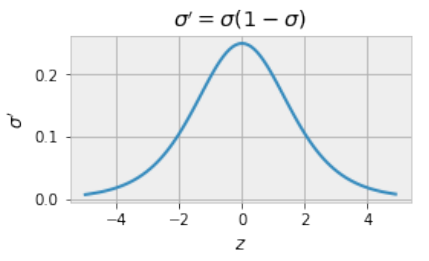
\includegraphics[scale=0.5]{../Figuras/devLog.png}
 \caption{Gráfica de la derivada de la función logistica.}
 \label{fig:graficaLogDev}
\end{figure}

Las funciones logísticas se utilizan a menudo en redes neuronales para introducir no linealidad en el modelo o para sujetar señales dentro de un intervalo específico . Un elemento de red neuronal popular calcula una combinación lineal de sus señales de entrada y aplica una función logística limitada como función de activación al resultado; este modelo puede verse como una variante "suavizada" de la neurona umbral clásica .

Estas relaciones dan como resultado implementaciones simplificadas de redes neuronales artificiales con neuronas artificiales. Las funciones sigmoidales que son antisimétricas con respecto al origen (por ejemplo, la tangente hiperbólica) conducen a una convergencia más rápida cuando se entrenan redes con retropropagación.

Una opción común para la activación o "aplastamiento" funciones, usadas para grandes magnitudes para mantener la respuesta de la red neuronal limitada. 

Las funciones logísticas se utilizan en varios roles en estadística. Por ejemplo, son la función de distribución acumulativa de la familia logística de distribuciones y, un poco simplificadas, se utilizan para modelar la posibilidad que tiene un jugador de ajedrez de vencer a su oponente en el sistema de clasificación.

En la siguiente sección veremos la derivada de la función de error.
